\documentclass[a4paper,14pt]{extarticle}
    \usepackage{amsmath}
    \usepackage{nccmath}
    \usepackage{amsfonts}
    \usepackage{lscape}
    \usepackage[utf8]{inputenc}
    \usepackage{titlepic}
    \usepackage{stackengine}
    \usepackage{lipsum}
    \usepackage{graphicx}
    \usepackage{booktabs}
    \usepackage{cite}
	\usepackage{caption}
	\usepackage{float}
	\usepackage{subcaption}
    \usepackage{multirow}
    \usepackage[top=1in, bottom=1.1in, left=1in, right=1in]{geometry}
    \usepackage{fancyhdr}
    \usepackage{relsize}
    \usepackage{tikz}
    \usetikzlibrary{shapes.geometric,arrows}
	\makeatletter
    \setlength{\@fptop}{0pt}
    \makeatother
    \tikzstyle{startstop} = [rectangle, rounded corners, minimum width = 4cm, minimum height=1cm, text centered,text width = 5cm, draw = black, fill=white!10]    
     \tikzstyle{process} = [rectangle,  minimum width = 4cm, minimum height=1cm, text centered, text width = 5cm,draw = black, fill = white!10]  
	 \tikzstyle{decision} = [diamond, minimum width = 4cm, minimum height=1cm, text centered,text width = 3cm, draw = black, fill = white!10]  
     \tikzstyle{arrow} = [thick,->,>=stealth] 
      
\begin{document}
\begin{center}
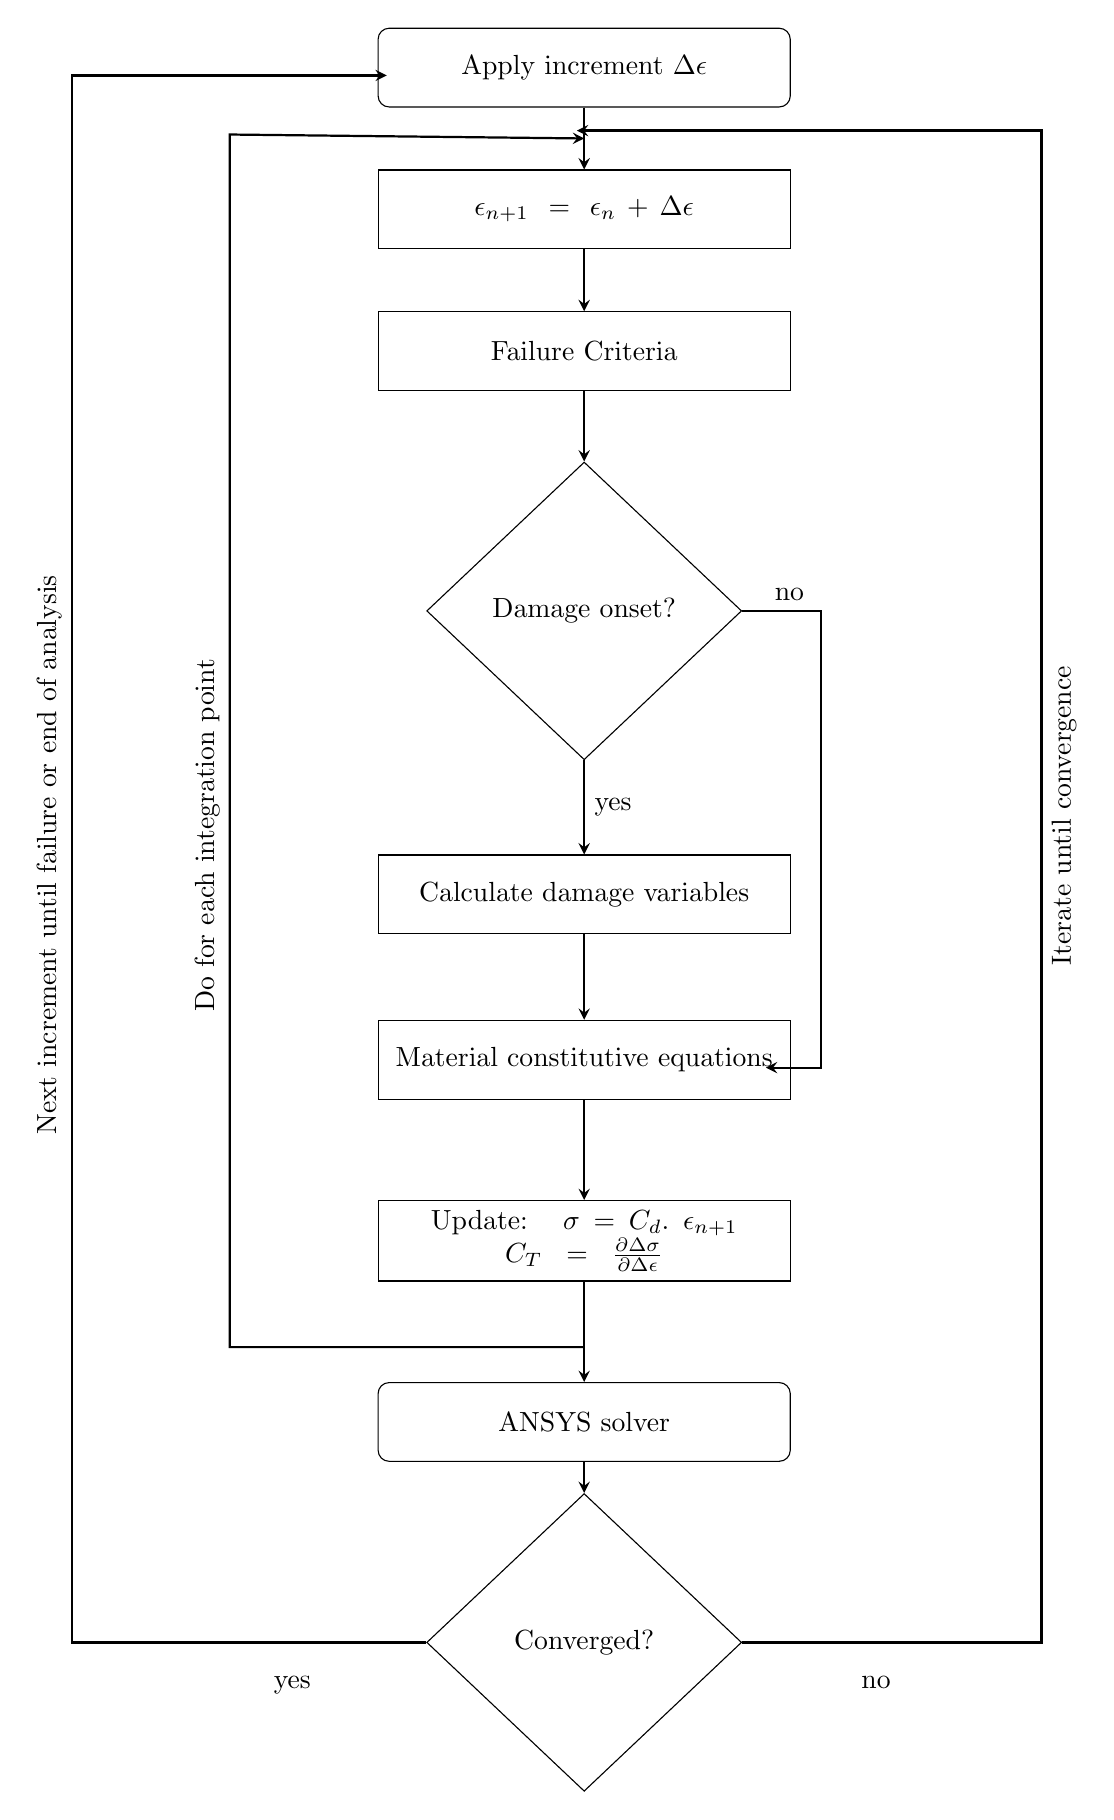
\begin{tikzpicture}[node distance = 1.8cm]

\node(straininc) [startstop] {Apply increment $\Delta\epsilon$};
\node(strainadd) [process, below of = straininc] {$\epsilon_{n+1} = \epsilon_{n} + \Delta\epsilon $};
\node(Failure)   [process, below of = strainadd] {Failure Criteria};
\node(Damageon)  [decision, below of = Failure, yshift=-1.5cm] {Damage onset?};
\node(Damagecalc) [process, below of = Damageon, yshift=-1.8cm] {Calculate damage variables};
\node(Materialeqn)[process, below of = Damagecalc, yshift=-0.3cm] {Material constitutive equations};
\node(Tangent)[process, below of = Materialeqn, yshift=-0.5cm] {Update: \; $\sigma = C_{d}.\; \epsilon_{n + 1}$ \\  $C_{T}=\frac{\partial \Delta \sigma}{\partial \Delta \epsilon}$};
\node(abaqus)[startstop, below of = Tangent, yshift=-0.5cm] {ANSYS solver};
\node(Converge)[decision, below of = abaqus, yshift=-1cm] {Converged?};

\draw [arrow] (straininc) -- (strainadd);
\draw [arrow] (strainadd) -- (Failure);
\draw [arrow] (Failure) -- (Damageon);
\draw [arrow] (Damageon) -- node[anchor = west]{yes} (Damagecalc);
\draw [arrow] (Damagecalc) -- (Materialeqn);
\draw [arrow] (Materialeqn) -- (Tangent);
\draw [arrow] (Tangent) -- (abaqus);
\draw [arrow] (abaqus) -- (Converge);
\draw [arrow] (Damageon.east) node[xshift=0.6cm,anchor = south]{no} -| ++(1,-5.8) -- ++(-0.7,0)  (Materialeqn);

\draw [arrow] (Converge.west)node[xshift=-1.7cm,yshift=-0.3cm,anchor = north]{yes} -| node[xshift=10cm,sloped,above]{Next increment until failure or end of analysis}++(-4.5,19.9) -- ++ (4,0) (straininc); 

\draw [arrow] (Converge.east)node[xshift=1.7cm,yshift=-0.3cm,anchor = north]{no} -| node[xshift=10.5cm,sloped,below]{Iterate until convergence} ++(3.8,19.2)-- ++ (-5.9,0)  (straininc); 

\draw [arrow] (0,-16.25)-|node[xshift=6.5cm,sloped,above]{Do for each integration point}++(-4.5,15.4)--(-0,-0.9);

 
\end{tikzpicture}
\end{center}
\end{document}